\section{Data Analysis Framework}\label{dataanalysisframework}

%\todo{Lägg till overall data table}

%Methods to choose from for analysing (i.e. what I did during the interactions, to test and analyze my app)

%Partly data collection done via app, but also all the observations

The results from each iteration needed to be analysed, see the previous figure \ref{studydesign}. Depending on the kind of activity and results gathered, different data is collected. For qualitative methods, the output is almost always notes and observations, which are then concluded into insights. These insights, can then sometimes be used in the below analysis methods. For quantitative data, the output is almost always \textit{quiz results} or data about the coaches. Before analysis, how this data has been processed is clearly described. Then, in the following sections, each data analysis methods is described.

%After this, an overview of which data analysis methods was used in what iteration is presented.

%\begin{itemize}
%\item Qualitative data
%\begin{itemize}
%\item Need groups and Personas (iteration \#1, constructed from stakeholder and coach interviews, field visits, and smartphone test)
%\item Customer Journey Map (iteration \#1, from workshop with coaches)
%\item Sprint backlog (iteration \#1, \#2, \#3, \#4, from feedback and observations during app tests, plus app design workshops)
%\item Sprint demo (iteration \#1, \#2, \#3, \#4, presenting quiz results and field visit findings)
%\end{itemize}
%\item Quantitative data (from quiz results and data about the coaches)
%\begin{itemize}
%\item Correlation in Google Sheets (iteration \#2, \#3, \#4)
%\item Correlation in R (iteration \#4)
%\item Logistical regression in R (iteration \#4)
%\item Parallel coordinates visualisation (iteration \#4)
%\end{itemize}
%\end{itemize}

\subsection{Data Analysis}\label{sec:data-analysis}

This section first presents relevant methods for analysing qualitative data, finally presenting analysing quantitative data. For analysing qualitative data in the research phase, Personas or Need groups are methods to analyse the though users of a product or a service. A Customer Journey Map supports understanding of how such users interact with a product or a service. Getting feedback from users involves getting ideas or suggestions for improvement of a product or a service. To analyse these, a sprint backlog is used to keep track of the priority of such feedback. If the features are then successfully implemented in the eyes of the users and stakeholders, can be tested using a sprint demo, where feedback is gathered for future work. These methods can be more closely read about below.

\subsubsection{Persona or Need groups}
When creating a product or a service, it is important to understand who you are designing for. Since the intended users might not always be around during the development phase, it helps having a clear mental image of the user. Fictional examples of users are one method to do this, either by using personas or need groups.  In this project, this is especially important, as a lot of development is off-site from the intended users, and the current author has no previous experience interacting with the intended users.

A \textit{persona} is a fictional character, created to give an example of the user who you are designing your service for \citep{stickdorn}. Depending on how broad the target group is for the service you are building, the persona might have several different needs. Then, dividing the though user groups in terms of designing for their different needs than their character traits might be more helpful \citep{expedition-mondial}. Dividing users by needs, if called forming \textit{need groups}. A need group (like "The beginner" or "The planner") can be described by their behaviour and their need. Personas and need groups should be developed from research insights gathered from interviews or workshops with users and stakeholders \citep{stickdorn}.

\subsubsection{Customer Journey Map}
A customer journey map is said to provide a vivid but structured visualisation of a service user's experience \citep{stickdorn}. A typical customer journey is multi-channel and time-based, see figure \ref{fig:cjmExample}. The customer journey map is beneficial both for understanding a user's touchpoints with a service, and also for collecting and analysing stories which explain why the journeys happened as they did \citep{stickdorn}. In this project, the Customer Journey Map is used to understand the activities that happens before, during and after having a youth session, and how these activities differentiate by different types of coaches (by persona and need group).

\begin{figure}[h]
    \centering
    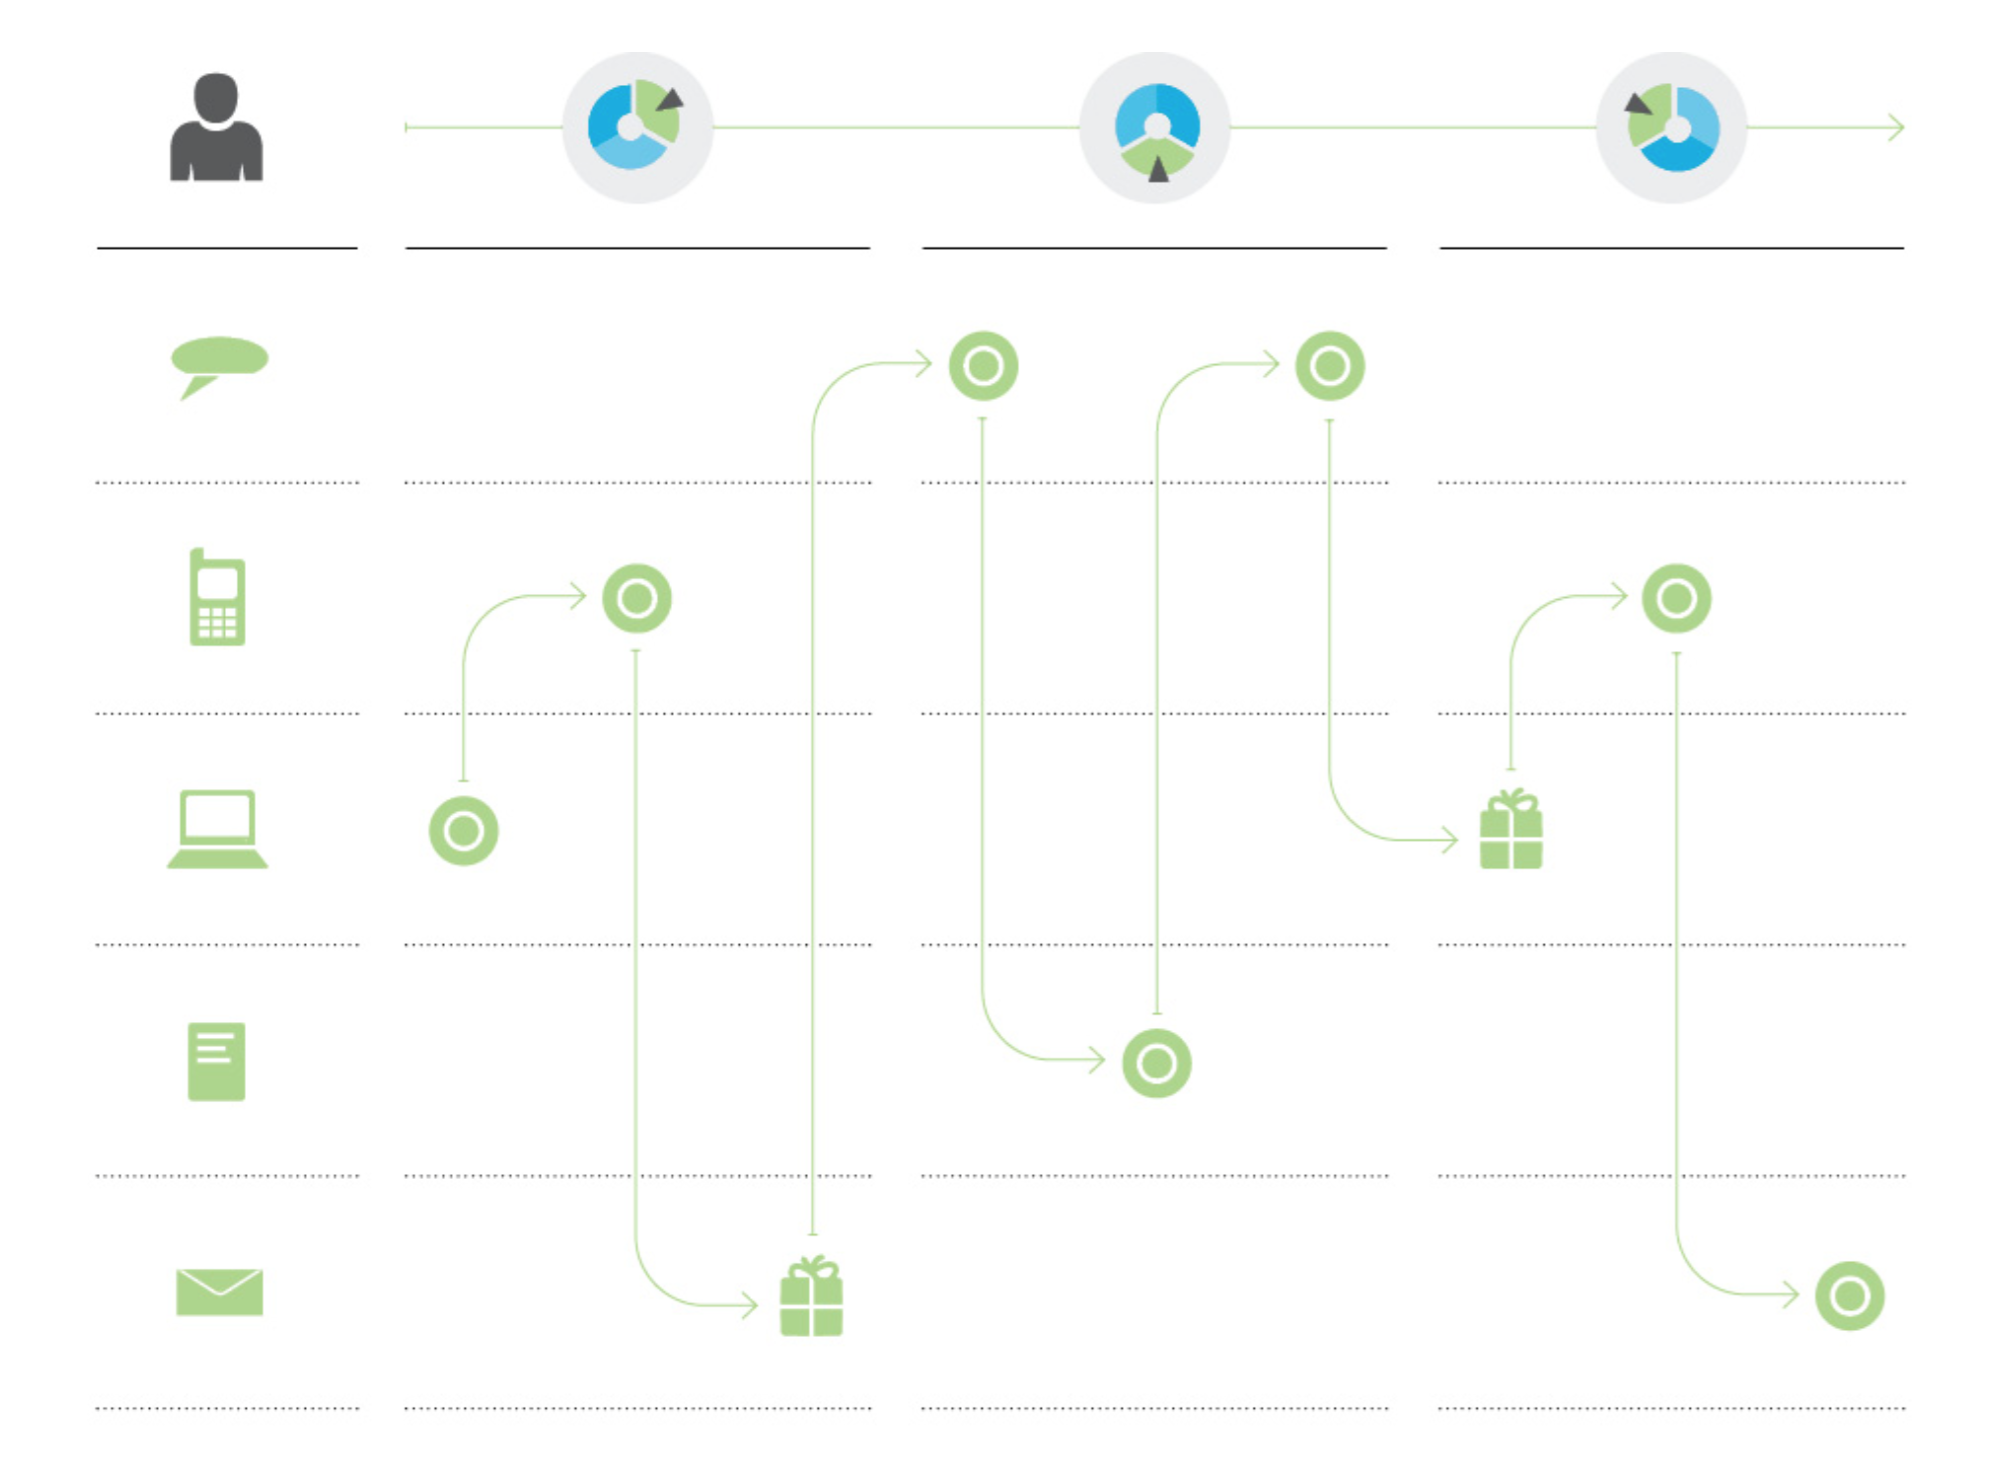
\includegraphics[width=0.7\textwidth]{analysis/cjmExample.png}
    \caption{General example of a customer service map. The map is divided by channel (could also be by a persona) and time (in this case before, during and after using a service).}
    \label{fig:cjmExample}
\end{figure}

\subsubsection{Sprint Backlog and Sprint Planning}
During product development, to do a \textit{sprint backlog} serves as a type of data analysis. When a high altitude of ideas and feedback has been gathered, a sprint backlog is a list sorted with the most important and urgent items on top. To work through ideas in a structured way, requests are categorized into what is called "stories". A good story answers "As a [user type] I want to be able to do [feature] so that [benefit]". Each story can then be broken down into tasks ("What needs to be done in order to satisfy the story?"). During the \textit{sprint planning}, at the start of each iteration, the most important stories and tasks are identified. By analysing and then working on the most prioritized story and task, you ensure that you are always working on what is most important for the success of the project. In this project, the sprint backlog is used to determine what actions needs to be prioritized in order to accomplish the goals set up during sprint planning.

At the end of an iteration, as much as possible of the sprint backlog has been taken from "Not done" to "Done". The things not done, are either moved into a product backlog (to later be added into an upcoming sprint backlog) or removed (they were not important enough).

\subsubsection{Sprint Demo}
A sprint demo is an effective way to analyse the product created after an iteration, from the perspective of the users and the stakeholders. \cite{kniberg} says that a well executed sprint demo attracts vital feedback from stakeholders, and ensures that tasks are 100\% done. A sprint demo does not need to be complicated: the product is shown and tested with users and stakeholders, getting feedback for the next iteration. But without it, it would not be possible to know if the work done has satisfied the needs of the end users, or what the stakeholders thinks is important for future work. The sprint demo in this project is evaluated both with stakeholders and the end target group, the coaches. Evaluation is done by the interaction design principles: desirability (does the coach desire to use the product?), utility (does it meet the needs of the coach?), usability (is the coach able to use it without frustration?) and pleasurability (is the coach satisfied using the product?) \citep{clatworthy}.

\subsubsection{Analysing Notes}
After an interaction, the notes (from interviews, workshops, tests and field visits) are transcribed from paper into the computer. This provides an opportunity to analyse the notes, think about their meaning and impact for the project, and categorize and separate notes that are comments from interviews (like a quote from a coach, which can help strengthen the description of a persona or a need group, or a feature suggestion that after analysis can be put into the product backlog) and insights from the current author, which can guide future development.

A \textit{mind-map} is usable for sorting and categorizing notes that are thoughts. In this project the interactive tool MindMeister \citep{mindmeister} is used. The tool has been used to sort through all interview notes and transcripts. Such an example include the evaluation interviews from iteration 4, that were divided into three different mind-maps: one fore learning, one for interaction design, and one for service design.

\subsubsection{Analysing Log Data}
Log data are often noted on paper during workshops and app tests. This includes the start time of a workshop, when and why a certain bug with the app appeared, or which coach chose to do an action in the app in a certain way. When these logs can help explain quiz results, they are often converted into comments in the Google Sheets where the quiz results are collected. This explains for example why iteration 4 has a coach that completed the coach quiz for week 9 for the summative test, but there are certain blanks in the Google Sheet: as the app did not record the expected data, the known log data was inserted into the Google Sheet.

\subsubsection{Analysing Test Items According to Bloom's Revised Taxonomy}
Using Bloom's Revised Taxonomy, the question from each quiz in the app can be evaluated by it's position on the knowledge dimension and the cognitive process dimension. Each question is given a "score", consisting of a letter and a number. The letter had the range of A-D for the knowledge dimension (A. "Factual", B. "Conceptual", C. "Procedural" and D. "Metacognitive") and the number had a range of 1-6 for the cognitive process dimension (1. "Remember", 2. "Understand", 3. "Apply", 4. "Analyze", 5. "Evaluate" and 6. "Create"). The data and comments are brought together into conclusions, to be presented during a sprint demo. In this project, this Bloom analysis is essential for being able to determine the learning effect of the test items.

\subsubsection{Analysing Quiz Results}
Below, methods for analysing collected quiz results and pre-test data in the project are presented. The first method used is correlation, but if multiple variables needs to taken into account, logistical regression can be used. As both of these are statistical tools, they rely on statistical significance in order to be trustworthy. In R programming language there are powerful tools for visualizing the correlation, for example using a "Correlation Heatmap", see figure \ref{fig:corrHeatmap}. In small-scale app tests, such amounts of data might not be sufficient.

To find trends or oddities in a small data set, visualization techniques to discover the quantitative data by hand might be more beneficial. To enable a visualization, data needs to be acquired, enhanced, mapped to a geometry and lastly rendered \citep{timo-ropinski-liu}. When rendered, a suitable rendering of a multiple-variable data set might be parallel coordinates, see figure \ref{fig:uneTerre}. Made interactive, each axis can be made filterable by user interaction.

\begin{figure}[h]
    \centering
    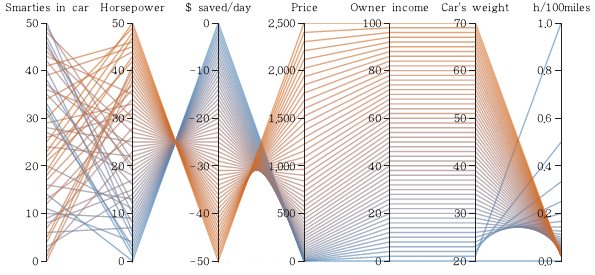
\includegraphics[width=0.7\textwidth]{analysis/terre.png}
    \caption{Parallel coordinates enables you to visually observe relationships and trends between dimensions: positive or negative relationship (correlation or invert), or no relationship at all (random) \citep{une-terre}}
    \label{fig:uneTerre}
\end{figure}

%\subsubsection{Calculating Correlation in Google Sheets and R}

%The process is to calculate and compare means on a "control"  with a response variable.

%It is clear that analysis in Google Sheets can only go so far. It can be greatly helpful to sort by multiple columns (e.g. first by Manual?, then by School level, then by Quiz 3). However, it takes a long time to filter the data on multiple parameters, and the work easily becomes tedious. For some applications, it may not be viable to discover the data using this approach.

%In Google Sheets, color scale can be used to give different column values different colors, see figure \ref{analysFarg4}. It is still hard to compare all of the axises towards all the axises, and it is not a scientific approach.

%Even in R, it is cumbersome to do statistically with all of the axises against all the axises. It is however possible to in both Google Sheets as well as the R programming language. Psuedo-code in R would be:

%\begin{verbatim}
%x1 = c(1,2,3,1,5,6)
%x2 = c(2,3,4,NA,6,7)
%cor(x = x1, y = x2)
%cor.test(x1,x2)
%\end{verbatim}

%In R programming language there are powerful tools for visualizing the correlation, for example using a "Correlation Heatmap", see figure \ref{fig:corrHeatmap}. %Psuedo-code in R would be:

%\begin{verbatim}
%random_matrix <- matrix(rnorm(100), nrow = 10, ncol = 10)
%random_matrix[1,1] <- NA
%colnames(random_matrix) <- paste("V",1:10)
%cor_mat <- cor(random_matrix)
%heatmap(cor_mat, keep.dendro = FALSE)
%\end{verbatim}

\begin{figure}[h]
    \centering
    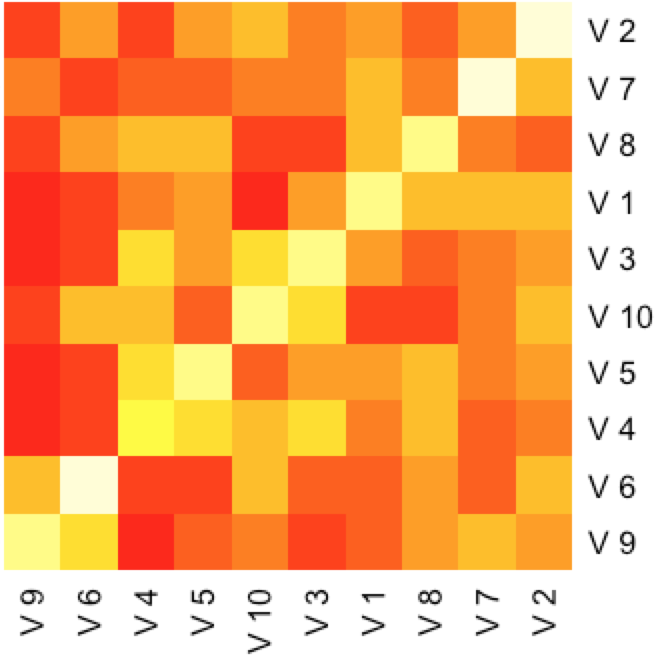
\includegraphics[width=0.45\textwidth]{analysis/rStatisticalAnalysis.png}
    \caption{A heatmap shows correlation  axis against axis. The more red a segment is, the bigger is the correlation between two axises. In this example there is a high correlation between for example V4 and V9. To be statistically significant in correlation or linear correlation, a common measure is that the Pr value ("the p-value") needs to be higher than 0.05 (meaning a 95\%+ probability).}
    \label{fig:corrHeatmap}
\end{figure}

\clearpage

%\subsubsection{Calculating Logistic Regression in R}

%A limitation with correlation is that only two dimensions can be compared with each other at the same time. What if we want to find a correlation between quiz score and gender \textit{and} age?

%To do this, Logistic Regression is helpful if our response variable can be a logistical dimension (e.g. women or male, used manual or not), while linear regression needs to be used if it is a linear or nominal scale (e.g. age and city respectively).

%In either case, the first step is to determine a response variable: the variable to compare against, e.g. is there a difference between men and women? In this case, it needs to be a quantitative measure of: "Have you learned anything?".

%If one more variable is added, e.g. also adding if a manual was used, this is called the "control". It is possible to add as many controls as possible.

%If linear regression, then it is needed to determine a quantitative measure of ("How much have you learned?").

%In Google Sheets, this is not effective to do. R, however, is a very suitable tool. First, the data is loaded, e.g. as a CSV file. Then, we tell R which the N/A values are, e.g. "N/A" or "Vet ej". We use this to filter the data. Then, each column we want to use is converted into a factor.

%When factors, a model can be created, e.g. using the General Linear Model. A different family can be selected, e.g. binomial.

%Then it is possible for R to show this data, showing the coefficient, the Pr value, and others. See code below.

%\begin{verbatim}
%mydata <- read.csv("Development/R/quizResults.csv", na.strings = c("N/A", "Vet ej"))

%mydata$y = ifelse(test = is.na(mydata$Quiz.9..y.n.1st),  yes = 0, no = 1)

%mydata$y <- as.factor(mydata$y)
%mydata$Help <- as.factor(mydata$Help)
%mydata$Sex <- as.factor(mydata$Sex)

%mymodel <- glm(formula = y ~ Pre.test.score + Sex, data = mydata, family = 'binomial')

%summary(mymodel)
%plot()

%\end{verbatim}

%For analysis, looking at the summary, coefficient (e.g. -1.0704) shows either a negative or positive correlation (in this case -7\%) for what to compare with as a response variable.

%To be significantly significant, a common measure is that the Pr value ("the p-value") needs to be higher than 0.05. If the p-value is higher than 0.05, it means that it is significant with a 95\% probability.

%\subsubsection{Visualizing and Analysing Multi-Variable Data with Parallel Coordinates}

%\cite{timo-ropinski-liu} describes the "visualization pipeline", generating an image from data:

%\begin{enumerate}
%\item Data acquisition ($\,\to\,$data are given)
%\item Data enhancement ($\,\to\,$ data are processed)
%\item Visualization mapping ($\,\to\,$ data are mapped to for example a geometry)
%\item Rendering ($\,\to\,$ images generated)
%\end{enumerate}

% Timo Ropinski, Scientific Visualization Group, Linköping University, TNM067 - Scientific Visualization, 9/12/2014)
% https://drive.google.com/drive/u/0/folders/0BzlK1PD8EE75bHIxcXRQNWpRMm8

%Data acquisition presents how data was acquired. Data enhancement explains how the data was processed. Visualization mapping is the process of mapping data to e.g. a geometry. Finally, rendering allows images to be generated, presented in 2D. This image can then be analysed.

%Parallel coordinates allows you to see relationships and trends between dimensions. They can be seen by a positive or negative relationship (correlation or invert), or no relationship at all (random) \cite{une-terre}. Parallel coordinates is not a quantitative data analysis per se, but it makes the data visually discoverable for visual analysis by a human. The human can more easily find patterns or outliers with a powerful visual representation.


%\subsection{Iteration 1: Uganda Coach Visit}

In iteration 1, the following activities were carried out and then analysed:

\begin{itemize}
\item Stakeholder interview (for Need groups)
\item Coach interview and field visit (for Need groups)
\item Workshop (for Customer Journey Map)
\item Smartphone test (for Need groups)
\end{itemize}

\subsection{Iteration 2: Zambia Coach Training}

In iteration 2, the following activities were carried out and then analysed:

\begin{itemize}
\item App test observations (for Sprint backlog)
\item Quiz results (for Sprint demo)
\item App design workshop: use case 1 (for Sprint backlog)
\item App design workshop: use case 2 (for Need groups)
\end{itemize}

\subsection{Iteration 3: Uganda Formative Test}

In iteration 3, the following activities were carried out and then analysed:

\begin{itemize}
\item App test observations (for Sprint backlog)
\item Service Mini-Sprint - 5 workshops (for Sprint backlog)
\item Field visits (for Sprint demo)
\item Small formative app test (for Sprint backlog)
\item Big formative app test (for Sprint demo)
\end{itemize}

\subsection{Iteration 4: Uganda Summative Test}

In iteration 4, the following activities were carried out and then analysed:

\begin{itemize}
\item Big summative app test (for Sprint demo and quantitative analysis)
\end{itemize}


\subsection{Analysis Implementation of Quiz Results and Pre-Data}

In this section, the steps needed to analyse the quantitative data is explained in detail, so that others can use a similar approach. In this example, quiz results are from iteration 4, but a similar approach has been taken with the manually recorded quiz results from iteration 2-3 as well.

Data analysis of quiz results was done first by a general overview in Google Sheets, by statistical analysis in R, and by a parallel coordinates visualization. The process to do this is described below.

\subsubsection{Step 1: Data Acquisition from Server}

It was desired to store the data in Google Sheets, thus it was necessary to collect the MongoDB database content, and convert JSON format into a Google Sheets-readable format, like CSV. Multiple approaches were tried, and the Google Chrome extension called Magic Json \citep{agaze} was the one that worked without problems.

\subsubsection{Step 2: Data Acquisition from Pre-Study}

The Pre-study data acquisition was done by instead of looking at the paper-submitted pre-study evaluation forms, using the data processed into Google Sheets.

\subsubsection{Step 3: Data Enhancement of Server Results}

This section presents how data from the server was processed, to enable visualization mapping. To make the data easier to work with, the columns were reordered, and made sortable and filterable. Some columns were given conditional formatting, so it would be easier to spot irregularities, see figure \ref{fig:resultsColored}. After this, some observations could be made.

\begin{figure}[h]
    \centering
    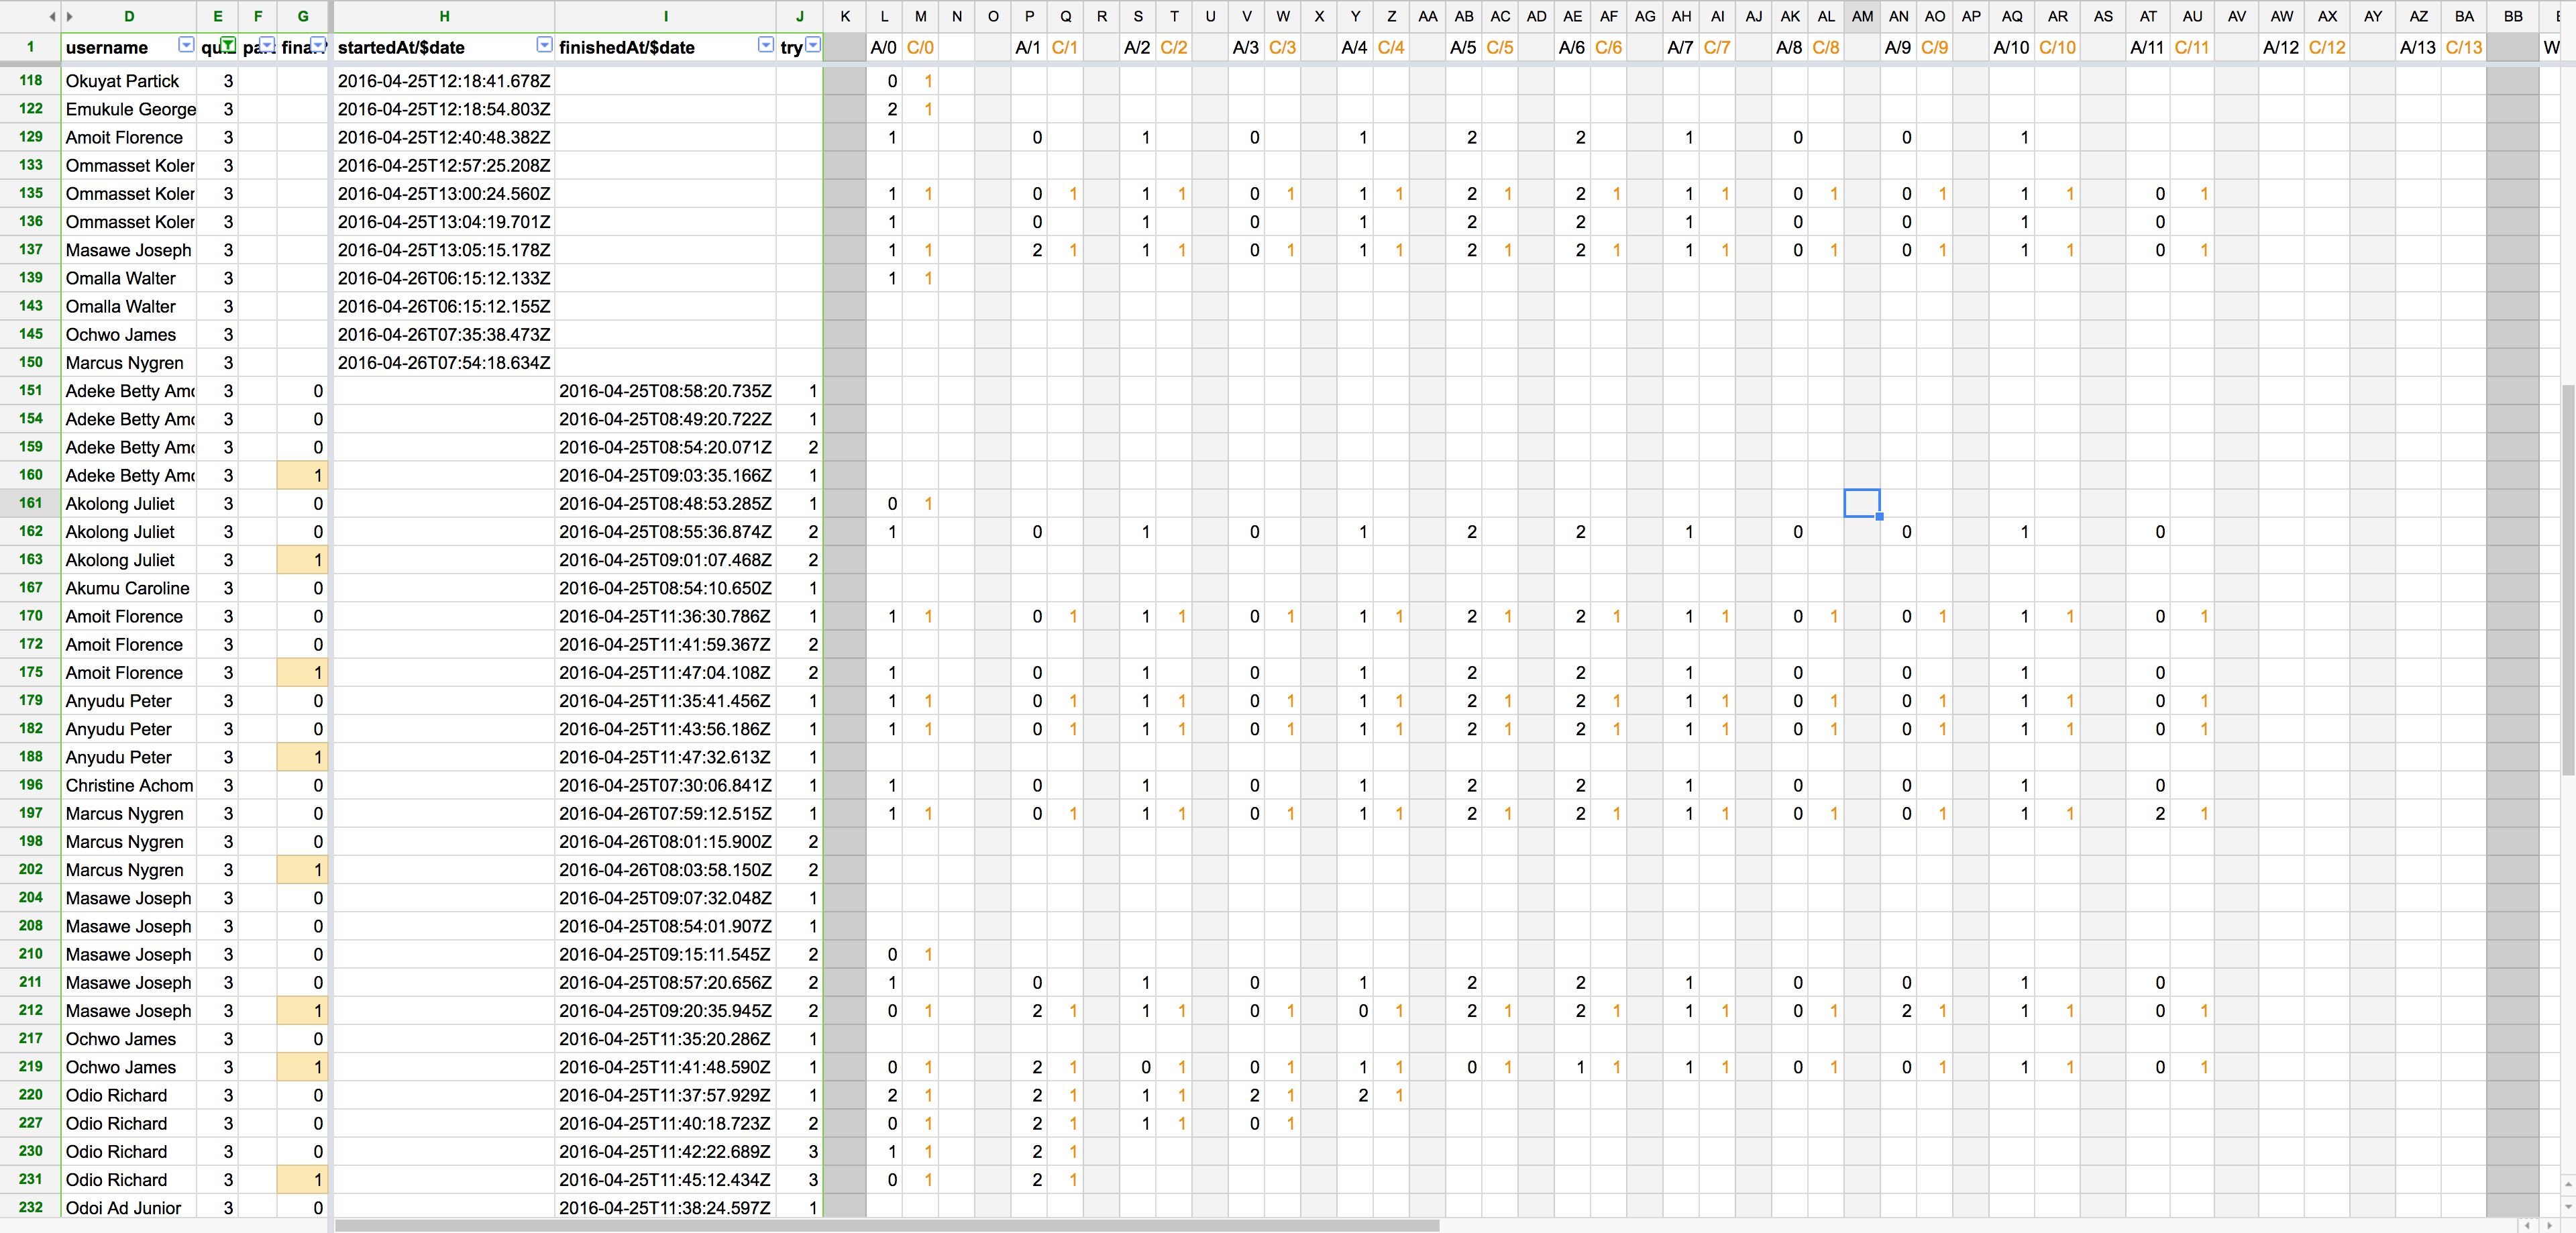
\includegraphics[width=0.9\textwidth]{analysis/resultsColored.png}
    \caption{The quiz results collected in a Google Sheet after data enhancement. In this figure, cell E1 has been filtered so that only results for quiz 3 are shown. Conditional formatting has been done with row G so that if it is a certification quiz, yellow color is used.}
    \label{fig:resultsColored}
\end{figure}

To be able to compare the test results with the pre-test results, it was clear that it would not be viable to test every dimension against every dimension. Instead, since goals of the app evaluation had been predefined in the following way, the quiz results were summarized into a new sheet so that the following could be derived:

\begin{itemize}
\item \% correct 1st try
\item number of tries until 100\%
\item number of tries until 100\% in 1 try
\end{itemize}

These could be calculated by having columns for:

\begin{itemize}
  \item Quiz 3
  \begin{itemize}
    \item Start time training
    \item \% correct 1st try
    \item number of tries until 100\% in 1 try
    \item Time difference start to end time certification
  \end{itemize}
  \item Quiz 9
  \begin{itemize}
    \item Start time training
    \item \% correct 1st try
    \item Time difference start to end 1st try
    \item Time difference start to passed training
    \item Time difference 1st try to certified
  \end{itemize}
\end{itemize}

Then, to see trends, color scales were again added. With ordinal values, a sequential color scheme is used (for example fastest time, from green to red), and with nominal values (like if they are female or male) where there is no right value, a qualitative color scheme is used. Now it was easier to spot outliers and trends, and giving validation to findings from notes and observations made during interviews, workshops and app tests.

\subsubsection{Step 4: Date Enhancement of Pre-study Results}
To see differences in answers more clearly, the data from the pre-study was made sortable and filterable. Then, the data was resampled for each column that had numerable (sortable) data in text instead of numbers, so for example "The day before" was changed to -1 and "The same day" to 0. In a similar way, school level was divided into four different groups, from 0 to 3, where 0 meant secondary, year unknown, 1 meant lower secondary, 2 meant upper secondary, and 3 meant tertiary.

After this, each column was given conditional formats using a color scale, using Google Sheets built-in functionality. This gave a visual way to quickly get an overview of the pre-test data.

\subsubsection{Step 5: Data Enhancement by Joining Pre-test and Results Summary}

The summary sheet and the pre-quiz sheet were joined, becoming a multiple-variate data set (several dimensions that were to bee compared with several other dimensions), see figure \ref{fig:analysFarg3}. A meeting with the university supervisors was held, so they could further give support in how to properly analyse the data. Since the two control groups showed similar means on the pre-quiz results, the two control groups were determined comparable.

\begin{figure}[h]
    \centering
    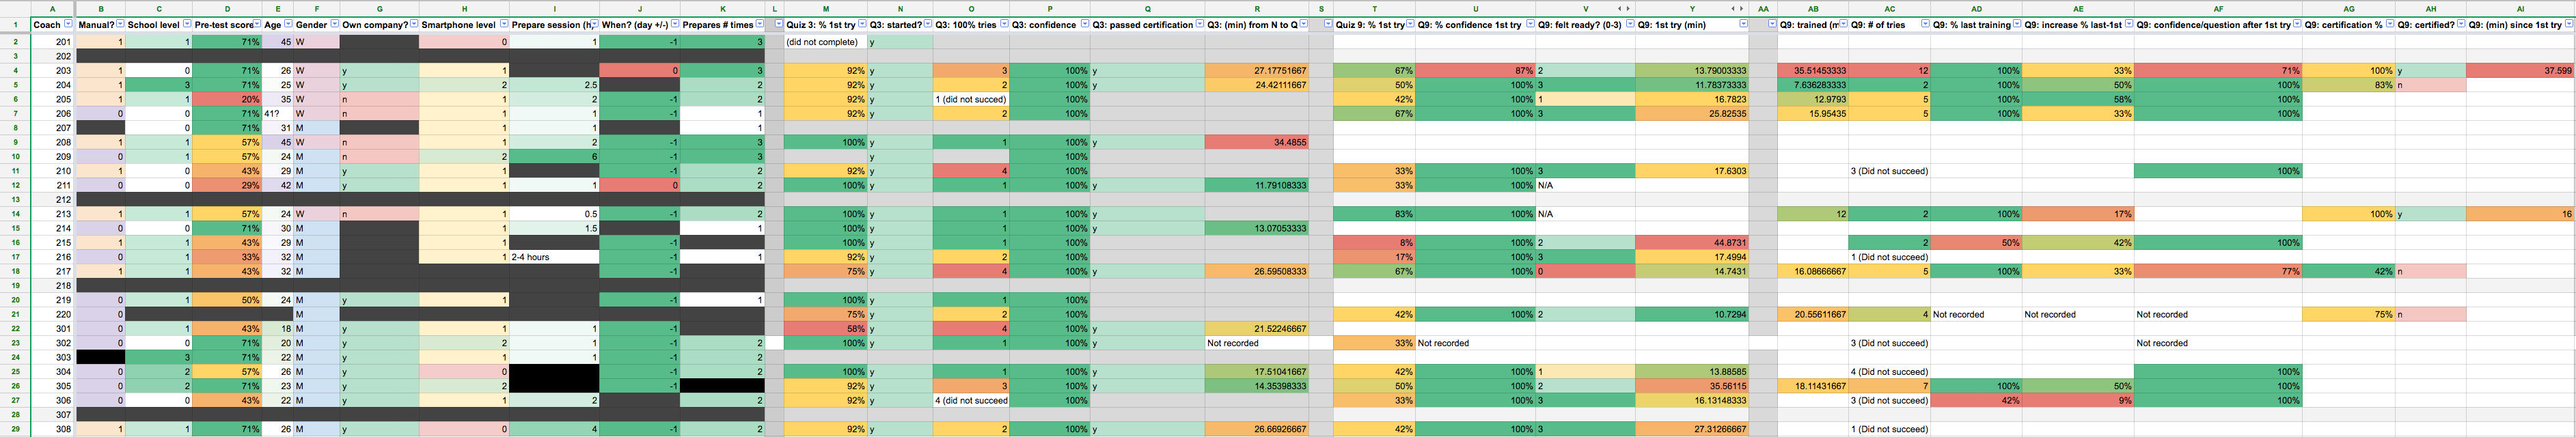
\includegraphics[width=1.0\textwidth]{analysis/sheets/0Overview.png}
    \caption{The multi-variate data set, made filterable and sortable in Google Sheets. Color scales and calculating means makes it easier to compare characteristics of the coach together with pre-test and quiz results. However, it is cumbersome and hard to quickly filter data on multiple parameters.}.
    \label{fig:analysFarg3}
\end{figure}

To meet the challenges of using Google Sheets, a multivariate analyzation software or a visualization was suggested to discover the data in less time. It was hard to determine a suitable multivariate analysis software suitable when having so few data points. Principle Component Analysis or Cohen's kappa would not be suitable, neither was it believed applicable to do Linear correlation on all dimensions. After discussion with other Master thesis students working with analysing data from various disciplines, parallel coordinates was suggested. It would allow very quickly filtering of the data, finding correlations, and distinguish outliers and common characteristics.

To guide the usage of the parallel coordinates (as there is so much to discover in the data set), using R to do Logistic correlation was also done. A disadvantage with this method, is that to be statistically significant, many data points may be needed, and it was now known before-hand if the method would be useful. Probably, parallel coordinates would be the best method to analyse a small multi-variate data set.

\subsubsection{Step 6: Visualization Mapping}
The goal with visualization mapping is to generate renderable data, in this case for the parallel coordinates visualization. Thus, a new spreadsheet is added, specific for visualizing the data. Columns were deleted that would serve no visual purpose (for example timestamps), gave all cells data values (even N/A when undefined), deleting users that did not have data, and shortened the column names so they would fit on the screen. The data was then exported from the Google Sheet into CSV.

\subsubsection{Step 7: Rendering}

For rendering, the JavaScript library D3.js, \citep{d3} was chosen. It supports data-driven documents for visualizing data with HTML, SVG and CSS. It supports both JSON and CSV data. A visual framework for multidimensional detectives for D3.js was found called "Parcoords.js", \cite{parcoords}. The example code from "Linking with a Data Table" provided the basis for the rendering. It allowed observing both the parallel coordinates visualization and the table data from the Google Sheet simultaneously.
% https://syntagmatic.github.io/parallel-coordinates/
% Chang, K. (2012). Parallel Coordinates toolkit : Parcoords.js 0.1. Parallel Coordinates toolkit. Retrieved September 8, 2012, from http://syntagmatic.github.com/parallel-coordinates/
% Kosara, R. (2010, May 13). Parallel Coordinates. Eagereyes.org. Retrieved September 8, 2012, from http://eagereyes.org/techniques/parallel-coordinates
% Tricaud, S. (2008). Picviz: finding a needle in a haystack. Proceedings WASL, San Diego. Retrieved from http://www.usenix.org/events/wasl08/tech/full_papers/tricaud/tricaud.pdf

 %https://syntagmatic.github.io/parallel-coordinates/examples/table.html

To work, the example CSV file was replaced with the data from exporting the Google Sheets data. To benefit the visualization, also the colors were changed, and the toolkit's functionality to drag the axes titles around to reorder the dimensions was used, since the goal was to quickly compare and find correlations. The result is visible in \ref{fig:parallell-coordinates-1}.

\begin{figure}[h]
    \centering
    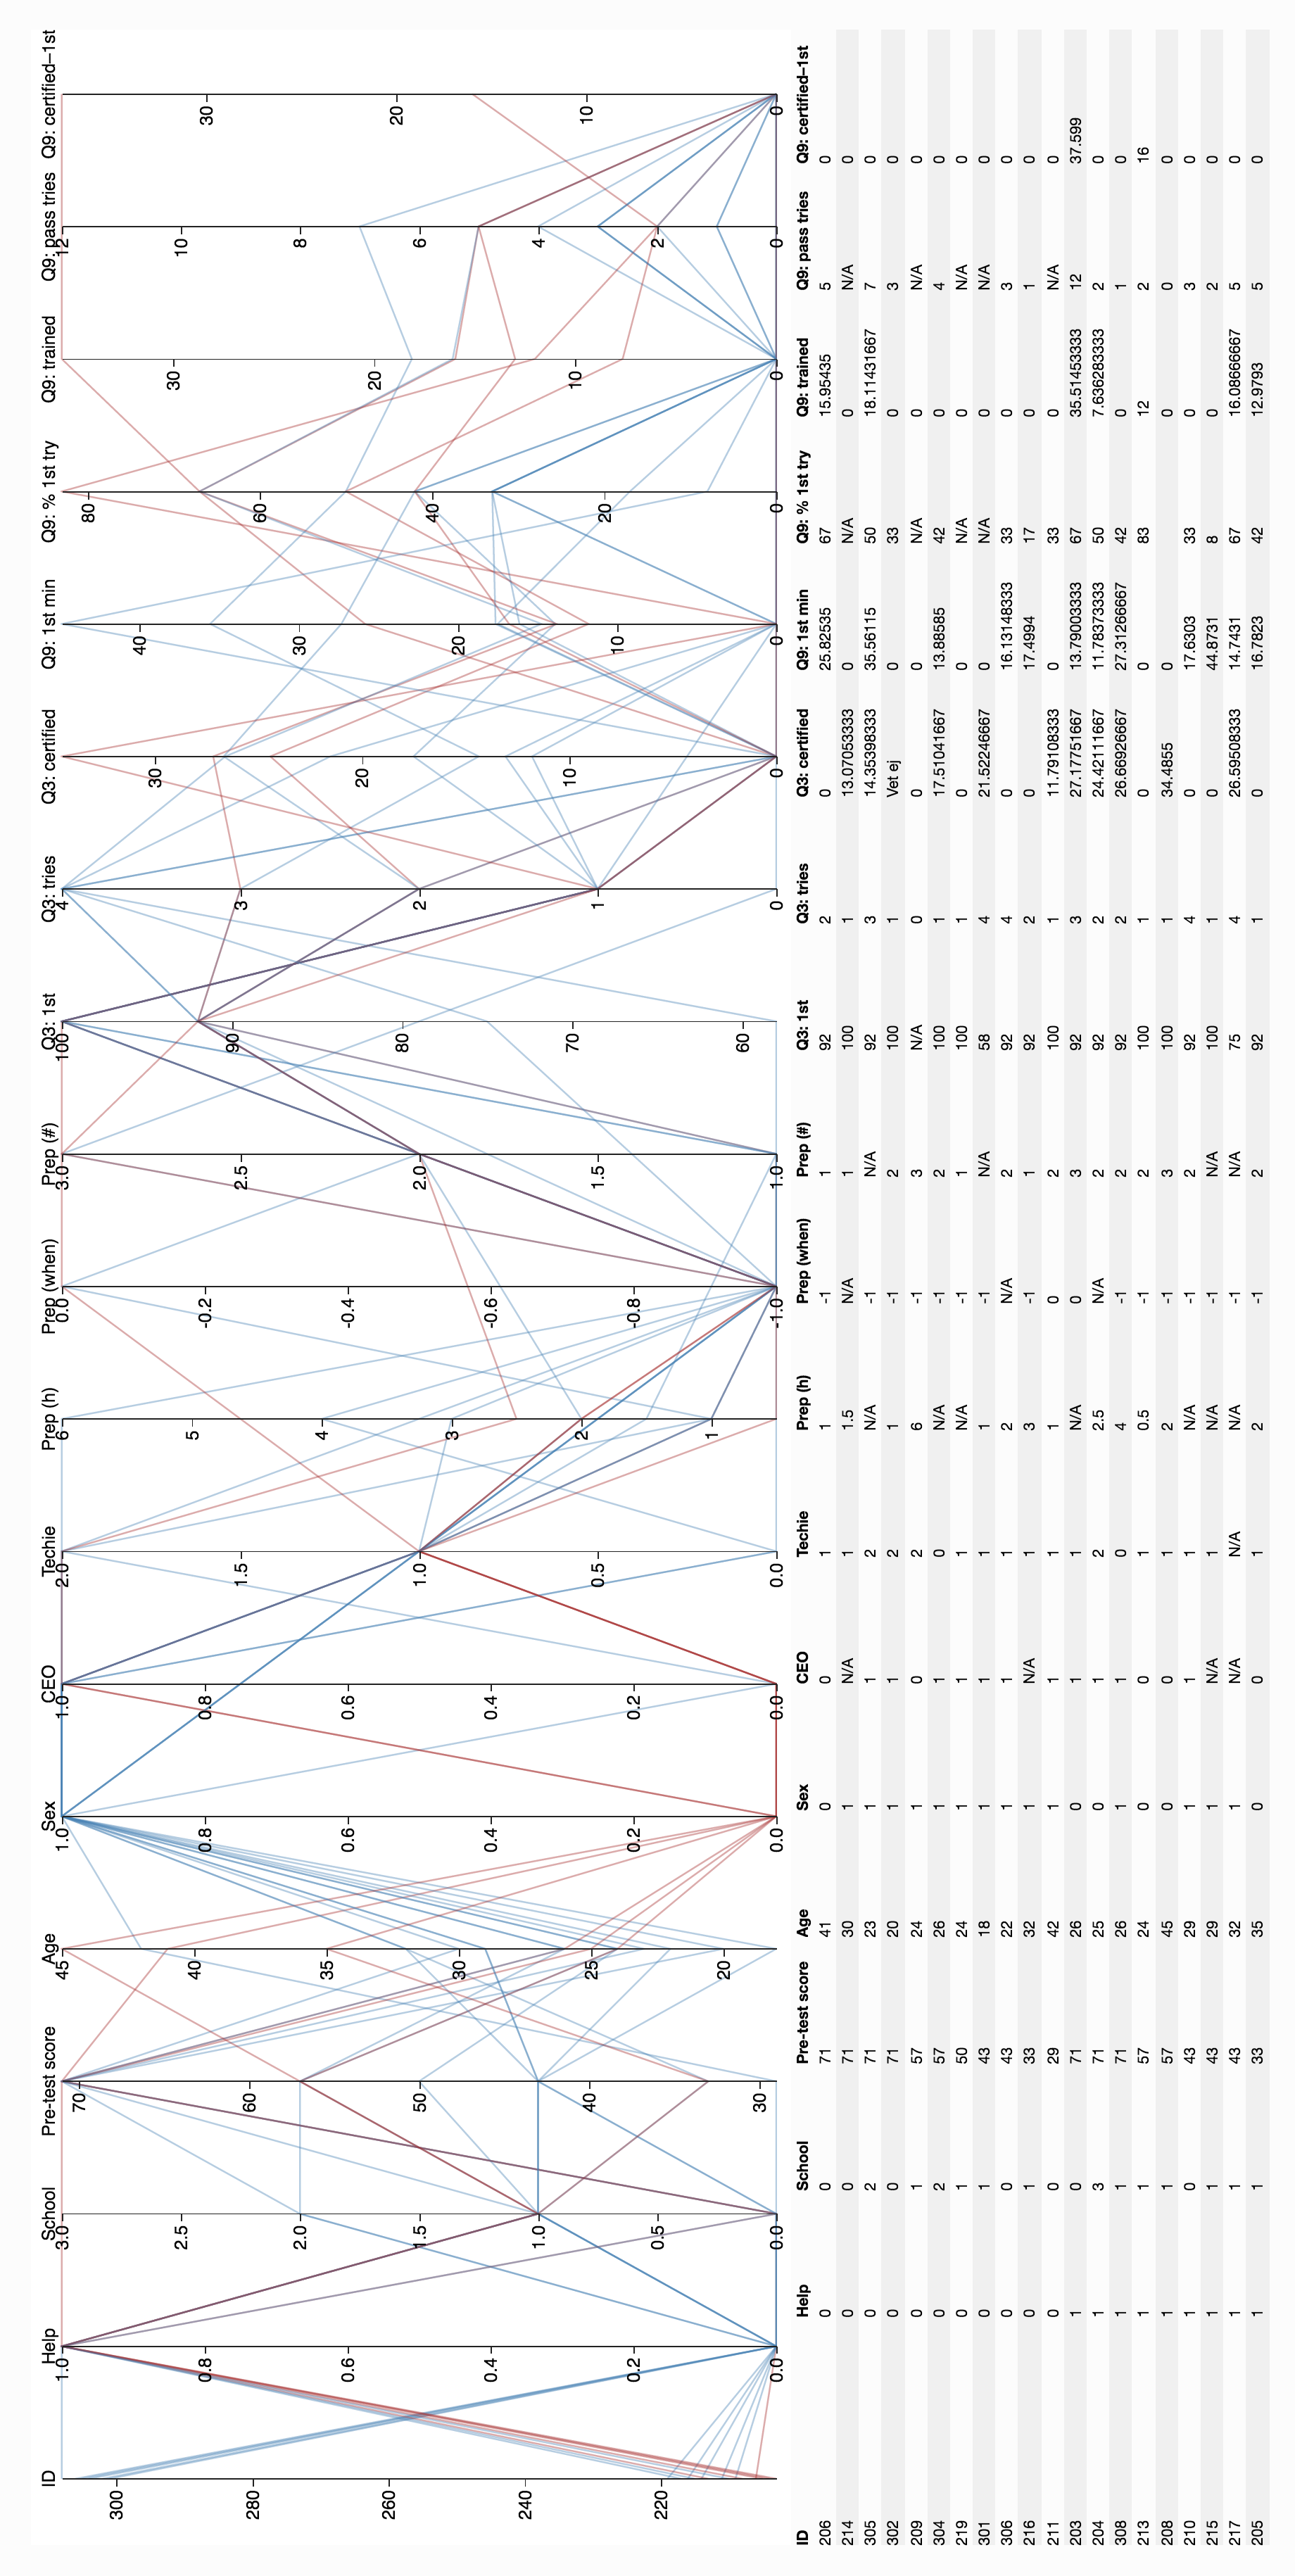
\includegraphics[width=0.7\textwidth]{analysis/parallellCoordinates3.png}
    \caption{The parallel coordinates visualization, done in d3.js. The visualization support draggable axes, filtering of data via dragging the sliders (which synchronizes with the data table), color assignment (like blue and red for men and women in the example), and hovering over a specific data point.}
    \label{fig:parallell-coordinates-1}
\end{figure}

